% = = = = = = = = = = = = = = = = = = = = = = = = = = = = = = = = = = = = = = = = = = = = =
% P  R  E  A  M  B  L  E
% = = = = = = = = = = = = = = = = = = = = = = = = = = = = = = = = = = = = = = = = = = = = =
\documentclass[11pt]{article}
\usepackage{amsbsy, amsmath, amssymb, authblk}

%\usepackage{array} 
%\usepackage{algorithm2e}
\usepackage{algorithmic}

\usepackage{booktabs, bm}
\usepackage[small,labelfont=bf,up,singlelinecheck=false]{caption}
\usepackage{cancel}
\usepackage{comment}
%\usepackage{fancyhdr}
%\usepackage[default]{lato}
\usepackage[T1]{fontenc}
\usepackage[bottom]{footmisc}
\usepackage{geometry}
\usepackage{graphicx}
\usepackage{hyperref}
%\usepackage[utf8]{inputenc}
%	\inputencoding{latin1}
%	\inputencoding{utf8}
%\usepackage{lettrine}
%\usepackage[sc]{mathpazo}
\usepackage{lmodern} % Nice fonts?
%\usepackage{mathrsfs}
\usepackage{mathtools} 
%\usepackage{marvosym} % silly bullet-point symbols (misc symbols)
%\usepackage{microtype}
\usepackage{minitoc}         % left in case it is needed elsewhere
\setcounter{secttocdepth}{5} % idem
\usepackage{etoc} % for toc before each section.
%\usepackage{multicol}
\usepackage{needspace}
\usepackage{paralist}
\usepackage{pifont}
%\usepackage{polynom} 			% typesetting polynomial long division
%\usepackage{setspace}
%	\onehalfspacing 
\usepackage{tocloft}
\usepackage{xparse} % DeclareDocumentCommand
\usepackage[compact]{titlesec} 		% compact shrinks whitespace around section headings.
\usepackage{ulem} 				% for strikeout \sout command.
%\usepackage{verbatim}

% Muh packagez :)
\usepackage{../../Packages/MathCommands}
\usepackage{../../Packages/BrandonColors}
\usepackage{../../Packages/BrandonBoxes}
\usepackage{../../Packages/NoteTaker}
\usepackage{../../Packages/CS221}

%\usepackage{program}
% DL BOOK CONVENTIONS
\renewcommand\vec[2][]{\bm{#2}_{#1}}

\DeclareDocumentCommand{\slice}
	{ O{t} O{1} m }
	{\vec[\langle #2 \ldots #1 \rangle]{#3}}

\newcommand\myfig[2][0.3\textwidth]{\begin{figure}[h!]\centering\includegraphics[width=#1]{#2}\end{figure}}
\newcommand\myspace[1][]{\vspace{#1\bigskipamount}\Needspace{10\baselineskip}}
\newcommand\p{\Needspace{10\baselineskip} \noindent}
\newcommand\tlab[1]{\tag{#1}\label{#1}}
\newcommand\Var[1]{\mathrm{Var}\left[#1\right]}

\usepackage{layout} % Type \layout() anywhere to see values of layout frame.
%\usepackage{showframe} % Displays layout frame on all pages
\usepackage{marginnote}
\renewcommand*{\marginfont}{\scriptsize}

\usepackage{listings}

\definecolor{dkgreen}{rgb}{0,0.6,0}
\definecolor{gray}{rgb}{0.5,0.5,0.5}
\definecolor{mauve}{rgb}{0.58,0,0.82}

\lstset{frame=tb,
	language=Java,
	aboveskip=3mm,
	belowskip=3mm,
	showstringspaces=false,
	columns=flexible,
	basicstyle={\small\ttfamily},
	numbers=none,
	numberstyle=\tiny\color{gray},
	keywordstyle=\color{blue},
	commentstyle=\color{dkgreen},
	stringstyle=\color{mauve},
	breaklines=true,
	breakatwhitespace=true,
	tabsize=3
}

\usepackage{tikz}
\usetikzlibrary{arrows, automata, shapes, snakes, positioning}
\usetikzlibrary{bayesnet}


\titleformat*{\subsubsection}{\small\scshape}
\newcommand\subsub[1]{\Needspace{15\baselineskip}\hrule\subsubsection{#1}\hrule}

% O{T} means "optional with default value of `T`"
% m means mandatory argument
\DeclareDocumentCommand{\vecseq}
	{ O{T} m }
	{ \{  \vec[1]{#2}, \ldots, \vec[#1]{#2}   \}  }
\DeclareDocumentCommand{\seq}
	{ O{T} m }
	{ \{ #2_1, \ldots #2_#1 \} }
	
\newcommand\QA[2]{\item \red{Q}: #1
	\begin{compactitem}
		\item \green{A}: #2
	\end{compactitem}}

%\setlength{\parskip}{1pt}
%\setlength{\columnseprule}{0.1pt}
%\setlength{\columnsep}{0.6cm}
%\setlength\tabcolsep{0.1cm}
\renewcommand{\arraystretch}{1.2}


\makeatletter
\newcommand*\dotp{\mathpalette\dotp@{.5}}
\newcommand*\dotp@[2]{\mathbin{\vcenter{\hbox{\scalebox{#2}{$\m@th#1\bullet$}}}}}
\makeatother

% --------------------------------------------------------------
% --------------------------------------------------------------

% Make all the ToC section/subsections small/condensed.
\renewcommand\cftsecfont{\small\bfseries}
\renewcommand\cftsubsecfont{\scriptsize}
\renewcommand\cftsubsubsecfont{\scriptsize}
\renewcommand\cftsecafterpnum{\vskip-5pt}
\renewcommand\cftsubsecafterpnum{\vskip-7pt}
\renewcommand\cftsubsubsecafterpnum{\vskip-7pt}

% bluesec
\newcommand\bluesec[1]{\myspace \p \blue{#1}}

\begin{document}
\dosecttoc
\tableofcontents




% ==================================================================================
% Lectures
% ==================================================================================
\mysection{Lectures}\label{Lectures}

% ------------------------------------------------------------------------------
\lecture{Lectures}{Machine Learning II}{April 09, 2019}

\p \blue{Roadmap}. 
\begin{compactitem}
	\item Features. 
	\item Neural Networks.
	\item Gradients without tears.
	\item Nearest Neighbors.
\end{compactitem}

\p \blue{Linear Classifiers}. Discussion of feature maps $\phi(x)$ that can be used for making a non-linear decision boundary \tstamp{52:00}.  

\myspace
\p \blue{Neural Networks}. 

\begin{example}[Predicting Car Collision \tstamp{58:00}]
Input: position of two oncoming cars $x = [x_1, x_2]$. 
 
Output: Whether safe ($y = +1$) or collide $y = -1$. 

We are told that the true function is
$$
y^* = \text{sign}(|x_1 - x_2| - 1)
$$
\tcblower

\begin{compactitem}

\item \textbf{Insight}: In $(x_1, x_2)$ space, there is a ``band'' (diagonal to the right centered about origin) representing ``safe'' \tstamp{58:30}. Recognize that these can be thought of as two linear decision boundaries.  

\item \textbf{Decompose} into subproblems\footnote{He is defining $\sign{0} \equiv -1$.}.
\begin{align}
	h_1 &= \ind{x_1 - x_2 \ge 1} \\
	h_2 &= \ind{x_2 - x_1 \ge 1} \\
	y &= \sign{h_1 + h_2}
\end{align}

\item \textbf{Learning strategy}. Define $\vec\phi(\vec x) \triangleq [1, x_1, x_2]$.
\begin{align}
	h_1
		&= \ind{\vec[1]{v} \dotp \vec\phi(\vec x) \ge 0  } 
		\qquad \vec[1]{v} \triangleq [ -1, +1, -1  ]   \\
	h_2	
		&= \ind{\vec[2]{v}  \dotp \vec\phi(\vec x) \ge 0 }
		\qquad
		\vec[2]{v} \triangleq [-1, -1, +1] \\
	f_{\matr V, \vec w}(\vec x)
		&= \sign{\vec w \dotp \vec h}
	\qquad
	\vec w \triangleq [1, 1]
\end{align}

\end{compactitem}

\red{Key idea: joint learning} \tstamp{1:03:42}. Learn both hidden subproblems $\matr V = (\vec[1]{v}, \vec[2]{v})$ and combination weights $\vec w = [w_1, w_2]$. \\
\end{example}

\myspace
\p \blue{Gradients}. (Continuing off example) Our parameters are $\{\vec[1]{v}, \vec[2]{v}, \vec w\}$. To learn these parameters, we may consider gradient descent on $y$ (and therefore on $h_1$ and $h_2$). Notice that
\begin{align}
\nabla_{\vec[1]{v}} h_1 = \vec 0 
\end{align}
Solution: Redefine $h_1 \triangleq \sigma\left( \vec[1]{v} \dotp \vec\phi(\vec x) \right)$. 

\myfig[0.3\textwidth]{figs/ml2_nn.png}


\myspace
\p \blue{Gradients without tears} \tstamp{1:14:00}. Gradients of common function building blocks:

\myfig[0.3\textwidth]{figs/ml2_building_blocks.png}


\myspace
\p \blue{Binary classification with hinge loss} \tstamp{1:17:01}. 
\begin{align}
L(x, y, w) 
&= \max\left\{
1 - \vec w \dotp \vec\phi(\vec x) y, 0
\right\}
\end{align}

\myfig[0.5\textwidth]{figs/ml2_backprop.png}



% ------------------------------------------------------------------------------
\lecture{Lectures}{Machine Learning III}{April 11, 2019}

\p \blue{Review}. Some feature extractor $\vec\phi(\vec x)$.
\begin{compactitem}
	\item Linear predictor score: $\vec w \dotp \vec\phi(\vec x)$. 
	\item Neural network score: $\sum_{j=1}^k w_j \sigma\left(  \vec[j]{v} \dotp \phi(x) \right)$. 
\end{compactitem}

\myspace
\p \blue{Generalization}. Goal is to minimize error on unseen future examples. 
\begin{compactitem}
	\item Suppose there is some space of all possible predictors $f$ and, within this space, there exists the optimal predictor $f^*$. 
	
	\item When we decide how we will do our feature extraction, we constrain the possible predictors we can get to be inside some \green{hypothesis class} $\mathcal F$ \tstamp{21:11}. Note that there exists a predictor $g$ that is optimal, constrained to being inside $\mathcal F$.  
	
	\item \green{Approximation Error}: How good is our hypothesis class $\mathcal F$? 
	
	\item \green{Estimation Error}: How good is our learned predictor $\hat f$ \textit{relative to} our hypothesis class $\mathcal F$?
	\graybox{
		\text{Err}(\hat f) - \text{Err}(f^*)
		&= \underbrace{ \text{Err}(\hat f) - \text{Err}(g) }_\text{Estimation} 
			+
			\underbrace{ \text{Err}(g) - \text{Err}(f^*) }_\text{Approximation}
	}
\end{compactitem}
\myfig[0.4\textwidth]{figs/ml3_err.png}

For linear predictors with weights $\vec w \in \R^d$, we can \textbf{control the size of $\mathcal F$} by \textellipsis
\begin{compactitem}
	\item Keeping dimensionality $d$ small.
	\begin{compactitem}
		\item Add/remove features.
		\item Forward selection.
		\item Boosting.
		\item $L_1$ regularization.
	\end{compactitem}
	\item Keeping the norm $|| \vec w ||$ small.
\end{compactitem}
Note that \green{SVMs} = hinge loss + regularization.\\

\p How do we choose \blue{hyperparameters} \tstamp{43:39}? One way is to use a \green{validation set}. 

\myspace 
\p \blue{Unsupervised Learning} \tstamp{1:06:00}. Data has rich \green{latent structures} that we'd like to learn automatically. Two types of unupervised learning: \green{clustering} (e.g. K-means) and \green{dimensionality reduction} (e.g. PCA). 

\begin{definition}{Clustering}
	\textbf{Input}: Training set of inputs $\mathcal{D}_{train} = \{ x_1, \ldots, x_n \}$.
	
	\textbf{Output}: Assignment of each point to a cluster $[ z_1 \ldots, z_n ]$ where $z_i \in \{1, \ldots, K\}$. 
\end{definition} 

\begin{algorithm}[K-Means Clustering \tstamp{1:10:35} ]
	\textbf{Setup}: Each cluster $k = 1, \ldots, K  $ is represented by a \green{centroid} $\vec[k]{\mu} \in \R^d$. Want each $\phi(x_i)$ close to its assigned centroid $\vec[z_i]{\mu}$. 
	
	\textbf{Objective}: MSE. 
	\begin{align}
		L(z, \mu)
			&= \insum || \phi(x_i) - \vec[z_i]{\mu} ||^2
	\end{align}
	
	\textbf{Algorithm}:
	\begin{compactenum}
		\item For each point $x_i$, assign:
		\begin{align}
			z_i := \argmin_{k=1,\ldots,K} ||\phi(x_i) - \mu_k||^2
		\end{align}
		
		\item For each cluster $k = 1, \ldots, K$, assign:
		\begin{align}
			\vec[k]{\mu} := \inv{| \{ i: z_i{=}k  \}   |}  \sum_{i: z_i{=}k} \phi(x_i)
		\end{align}
	\end{compactenum}
\end{algorithm}




% ------------------------------------------------------------------------------
\lecture{Lectures}{Search I}{April 16, 2019}

Running example: farmer has a boat. Needs to get a cabbage, goat, and wolf across river. Goat and cabbage cannot be alone. Wolf and goat cannot be alone. Boat can hold at most two things (including farmer). How he do it tho?

\p \blue{Beyond Reflex} \tstamp{9:00}. Classifiers (reflex) map $x$ to single action $y$. In \green{search}, we map $x$ to an \textit{action sequence} $(a_1, a_2, \ldots)$. \textbf{Key}: Need to consider consequences of future actions. 

\myspace
\p \blue{Tree search}. Root note is start state. Edges are actions. Nodes are states resulting from said action. Branches represent a sequence of actions. 
\begin{compactitem}
	\item $S_{start}$ is "FCGW|" (farmer, cabbage, goat, wolf all on left of river). 
	\item Actions: farmer can go to/from river. Actions enumerate what he takes with him and what direction he goes. 
	\item Cost(s, a): ?
	\item Succ(s, a): returns the state resulting from taking action $a$ from state $s$. 
	\item IsEnd(s): ?
\end{compactitem}

\begin{example}[Transportation example \tstamp{17:40}]
	\textit{Streets with blocks numbered $1$ to $n$. Walking from $s$ to $s+1$ takes 1 minute. Taking a magic tram from $s$ to $2s$ takes 2 minutes. How to travel from $1$ to $n$ in the least time?}
	
	\tcblower 
	
	You should read this and then try formalizing it as a search problem.
	\begin{compactitem}
		\item Actions: either take 1 step forward or take the tram.
		\item The costs are 1 minute and 2 minutes for the aforementioned actions.
	\end{compactitem}


	She starts coding it up at \tstamp{19:30}. Takeaways from coding:
	\begin{compactitem}
		\item Separate modeling from inference. 
		\item Modeling: She defines a class with methods startState, isEnd(state), succAndCost(state). 
	\end{compactitem}
\end{example}

\myspace
\p \blue{Backtracking search} \tstamp{23:10}. Also uses a search tree. Define branching factor $b$ and depth $D$ of tree\footnote{Distinguishing between uppercase $D$ and lowercase $d$ will be important in this lecture.}. BS goes down all the way leftmost to leaf. Sounds like \green{depth-first search} tbh\footnote{At \tstamp{34:00} she address this. Yes, it is basically DFS, but DFS will \textit{stop} as soon as it hits a leaf (a solution). Also, DFS implicitly defines all costs as zero.}
\begin{compactitem}
	\item Memory: $\mathcal O(D)$ (small). Why? because we only need to remember our past history, which for BS is basically a straight line from leaf back up to root. 
	
	\item Time: $\mathcal O(b^D)$ (huge). In other words, all nodes. Why? because worst-case is that it has to visit every single node. 
\end{compactitem}

\myspace\Needspace{10\baselineskip}
She starts coding for BS at \tstamp{27:28}. Note that she is able to reuse her code from the previous part, where she just defined the \textit{model}. Now, she implements BS which is the \textit{inference}. Below is the BS \textit{algorithm}\footnote{Which is slightly different in form than her code.}:
\begin{lstlisting}[language=Python]
def backtracking_search(s, path):
	if is_end(s):
		minimum_cost_path = min(minimum_cost_path, path)
	
	for a in actions(s):
		path.append([succ(s, a), cost(s, a)])
		backtracking_search(Succ(s, a), path)
	
	return minimum_cost_path
\end{lstlisting}

\myspace
\p \blue{Breadth-first Search} \tstamp{37:00}. Requires that cost for all actions is the same constant $c \ge 0$. Explores level-by-level. Like DFS, terminates as soon as it finds a solution\footnote{This is a consequence of the fixed global cost $c \ge 0$.}. Important: let $d$ (small d) denote the depth of the \textit{solution}. 
\begin{compactitem}
	\item Memory: $\mathcal O(b^d)$ (a lot worse!).
	\item Time: $\mathcal O(b^d)$ (better, depends on $d$, not $D$).
\end{compactitem}

Brief overview of \green{DFS with iterative deepening} at \tstamp{41:00}. Hybrid of DFS with BFS. Call DFS at max depths 1, 2, $\ldots$ etc. $\mathcal O(d)$ space and $\mathcal O(b^d)$ time. Nice summary slide of tree search algorithms at \tstamp{43:11}. 

\myspace 
\p \blue{Dynamic programming} \tstamp{43:30}. Observation: the cost of going from $s$ to end state can be decomposed into cost of $(s, a) \rightarrow s'$ plus the cost of going from $s'$ to end state.
\begin{compactitem}
	\item Denote ``future cost'' of state $s$ as $F(s)$. 
	\begin{align}
		F(s) \triangleq 
		\begin{cases}
			0 & IsEnd(s) \\
			\min_{a \in Actions(s)} C(s, a) + F(Succ(s, a)) & \text{otherwise} 
		\end{cases}
	\end{align}
	
	\item \textbf{Key observation}: \textit{we can cache intermediate results}. 
	
	\item \textbf{Assumption}: State graph defined by $Actions(s)$ and $Succ(s, a)$ is acyclic. 
	
	\item State should be sufficient to encode full history, so that futureCost(state) can be computed. 
\end{compactitem}

\myspace\Needspace{15\baselineskip}
\begin{example}[Route finding \tstamp{47:38}]
	\textit{Find minimum cost path from city $1$ to $n$, only moving forward. It costs $c_{ij}$ to go from $i$ to $j$.}
	\tcblower 
	Clarification: Yeah, you can go from any $i$ to $i + j$ for $0 \le j \le n - i$. 
	\textbf{Observation}: future cost only depends on the current city (since we can only move forward). Cache, cache, cache.\\
	
	What if we add the \textbf{constraint} that you can't visit three odd cities in a row. How does this change our definition of a state? Well, now we need to encode history somehow. 
	\begin{compactitem}
	\item Naive: redefine our state as (prev city, current city). This increases our state space size from $n$ to $n^2$. 
	
	\item More compact: redefine our state as (prevWasOdd, current city). Now our state space is $2n$. 
	\end{compactitem}
\end{example}

\myspace\Needspace{10\baselineskip}
Coding for dynamic programming:
\begin{lstlisting}[language=Python]
def dynamic_programming(problem):
	cache = {}  # state -> future_cost(state)
	def future_cost(state):
		if problem.is_end(state):
			return 0
		if state in cache:
			return cache[state]
		result = min(cost + future_cost(new_state) for _, new_state, cost in problem.succ_and_cost(state))
		cache[state] = result
		return result
	return future_cost(problem.start_state(), [])
\end{lstlisting}


\myspace
\p \blue{Uniform cost search} \tstamp{1:05:00}. Can handle cycles. 
\begin{compactitem}
	\item \textbf{Assumption}: $\forall (s, a): C(s, a) \ge 0$. 
	
	\item \textbf{Observation}: prefixes of optimal path are optimal. 
	
	\item \textbf{Key idea}: Enumerate states in order of increasing past cost. 
\end{compactitem}


\begin{center}
	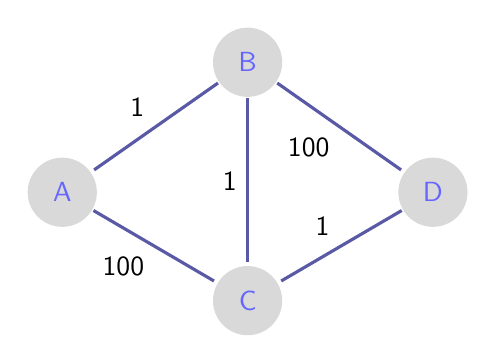
\begin{tikzpicture}[font=\sffamily,node distance=1.cm,->,>=latex,auto,line width=0.4mm]
	
	
	\tikzset{node st/.style={state, draw=none,
			fill=gray!30!white,
			text=blue!60!white}}
	\tikzset{node obs/.style={state, draw=none,
			fill=gray!60!black,
			text=blue!20!white}}
	
	\node[node st] (A) {B};
	\node[below=3em of A] (dummy) {};
	\node[node st, left=5em of dummy] (D) {A};
	\node[node st, right=5em of dummy] (B) {D};  
	\node[node st, below=6em of A] (C) {C};
	
	\draw[every loop,auto=right,draw=blue!30!gray]
	(A) edge[-] node{100} (B)
	(A) edge[-] node{1} (D)
	(A) edge[-] node{1} (C)
	(B) edge[-] node{1} (C)
	(D) edge[-] node{100} (C);
	\end{tikzpicture}
\end{center}
Goal: Use UCS to get from A to D. 
\begin{compactitem}
	\item Maintain 3 sets of states: explored, frontier, and unexplored.
	\item We start with all states in the unexplored sets. 
	\item Pop A into the frontier. What states can we reach from A? 
	\item Pop B and C into frontier and the cost to get to them. A is now in the explored set. 
\end{compactitem}
It seems we don't explore states we've already been to? UCS is \textit{correct}: when any state $s$ is moved from frontier to explored, its priority of $PastCost(s)$ is the minimum cost to $s$ (discussion around \tstamp{1:18:00}). 

\myspace
Coding for UCS begins at \tstamp{1:15:00}. 

\begin{lstlisting}[language=Python]
def uniform_cost_search(problem):
	frontier = PriorityQueue()
	frontier.update(problem.start_state(), 0)
	
	while True:
	# Move from frontier to explored.
	state, past_cost = frontier.remove_min()
	if problem.is_end(state):
		return past_cost, []
	# Push out onto frontier.
	for a, new_state, cost in problem.succ_and_cost(state):
		frontier.update(new_state, past_cost + cost)
\end{lstlisting}

\myfig[0.4\textwidth]{figs/search_ucs.png}





% ------------------------------------------------------------------------------
\lecture{Lectures}{Search II}{April 18, 2019}

\p Discussion of \textbf{Final Project} up until \tstamp{15:00}. 

\myspace
\p \blue{Review}. \textbf{Key idea}: a \green{state} is a summary of all the past actions sufficient to choose future actions \textbf{optimally}. The class paradigm includes modeling, inference, and learning. Today will talk more about learning. 

\myspace
\p \blue{Learning costs} \tstamp{25:00}. What if we don't have access to the costs? Goal: develop a learning algorithm that outputs the costs of actions.  
\graybox{
	\text{\footnotesize Forward problem \textbf{(Search)}} \quad 	
		\mblue{Cost(s, a)} &\longrightarrow \mred{(a_1, \ldots, a_k)} \\
	\text{\footnotesize Inverse problem \textbf{(Learning)}} \quad
		\mred{(a_1, \ldots, a_k)} &\longrightarrow \mblue{Cost(s, a)}
}

Prediction (inference) problem:
\begin{compactitem}
	\item Inputs (x): search problem without costs.
	\item Outputs (y): sequence of optimal actions.
\end{compactitem}
So our training data is search problem inputs and the labeled solutions (action sequence) for each. We need to learn that mapping from search problem to optimal action sequence. The idea is that we'll learn the costs by doing this. A simple way of modeling this\footnote{Note that $w$ does not care about the state we are taking the action from.}:
\begin{align}
	Cost(s, a_i) &\triangleq w[a_i] \triangleq w_i 
\end{align}

\begin{algorithm}[Structured Perceptron (simplified) \tstamp{32:00}]
	\begin{compactenum}
		\item For each action $a$, initialize $w[a] \leftarrow 0$. 
		
		\item For each iteration $t = 1, \ldots, T$:
		\begin{compactenum}
			\item For each $(x, y) \in \mathcal D_{train}$:
			\begin{compactenum}
				\item Compute minimum cost path $y'$ given $\vec w$. 
				\item $\forall a \in y: w[a] \leftarrow w[a] - 1$. 
				\item $\forall a \in y': w[a] \leftarrow w[a] + 1$. 
			\end{compactenum}
		\end{compactenum}
	\end{compactenum}
\end{algorithm}
Coding for this starts at \tstamp{38:00}. It just uses a modified version of TransportationProblem (model) that incorporates weights, and uses the dynamicProgramming function (inference) unchanged. Then it updates weights as defined above. \\

\p \blue{Generalization to features} \tstamp{46:10}. Costs are parameterized by [incorporating] a feature vector:
\begin{align}
	Cost(s, a) &= \vec w \dotp \phi(s, a) \\
	Cost(y) &= \vec w \dotp \sum_{(s, a) \in y} \phi(s, a)
\end{align} 

\myspace
\p \blue{A* search} \tstamp{46:30}. Improving upon UCS:
\begin{compactitem}
	\item \textbf{Problem}: UCS orders states by cost from $s_{start}$ to $s$. 
	\item \textbf{Goal}: take into account cost from $s$ to $s_{end}$. 
\end{compactitem}
Since we obviously don't know $FutureCost(s)$, A* will explore in order $PastCost(s) + \mred{h(s)}$, using a \green{heuristic function} that estimates future cost. 
\graybox{
	\underbrace{Cost'(s, a)  }_{\text{A*}}
		&= \underbrace{ Cost(s, a) }_{\text{UCS}} 
			+ h\left(  Succ\left(   s, a  \right)  \right) - h(s)
}
\begin{compactitem}
	\item \textbf{Consistency of $h$}. A heuristic $h$ is \green{consistent} if both of the following hold:
	\begin{align}
		Cost'(s, a) &\ge 0 \\
		h(s_{end}) &= 0
	\end{align}
	\myfig[0.3\textwidth]{figs/search2_consistency.png}
	
	\begin{definition}[0em]{Proposition: Correctness of A* \tstamp{56:40}}
		If $h$ is consistent, A* returns the minimum cost path\footnote{Proof hint: show that A* ultimately ends up returning UCS + a constant after you sum everything up.}.
	\end{definition}

	
	\item \textbf{Admissibility of $h$} \tstamp{1:02:20}. A heuristic $h$ is admissible if
	\begin{align}
		h(s) \le FutureCost(s)
	\end{align} 
	Intuition: admissible heuristics are \textit{optimistic}. Theorem: $isConsistent(h) \Rightarrow isAdmissible(h)$. 
\end{compactitem}

\myspace 
\p \blue{Efficiency}.
\begin{compactitem}
	\item UCS efficiency: UCS explores all states $s$ satisfying $$PastCost(s) \le PastCost(s_{end})$$. 
	
	\item \red{A* efficiency: A* explores all states $s$ satisfying $$PastCost(s) \le PastCost(s_{end}) - h(s)$$.}\footnote{IDGI. Plz explain here when smarter.}
\end{compactitem}

\myfig[0.6\textwidth]{figs/search2_astar_explore.png}

\Needspace{10\baselineskip}
\begin{definition}{Key Idea: \green{distortion} \tstamp{1:02:00}}
	\red{A* distorts edge costs to favor end states.}
\end{definition} 



\myspace
\p \blue{Relaxation} \tstamp{1:04:00}. How we find heuristics. Basically, removing constraints. 













% ------------------------------------------------------------------------------
\lecture{Lectures}{Markov Decision Processes}{April 23, 2019}

\p \blue{Motivation}. (Building off search problems) There is \textbf{uncertainty} in the world. Volcano crossing example starts at \tstamp{7:20}. 

\begin{example}[Dice Game \tstamp{13:12}]
	For each round $r = 1, 2, \ldots$
	\begin{compactitem}
		\item You choose to \green{stay} or \red{quit}. 
		\item If \red{quit}, you get \$10 and end the game.
		\item If \green{stay}, get \$4 and then roll a 6-sided dice. 
		\begin{compactitem}
			\item If result is 1 or 2 $\rightarrow$ end game.
			\item Otherwise, continue to next round.
		\end{compactitem}
	\end{compactitem}

	\tcblower

	Train of thought should roughly go as follows:
	\begin{compactitem}
		\item If I follow policy \green{stay}, I can compute my expected reward as
		\begin{align}
			\inv{3} (4) + \frac{2}{3}\inv{3} (8) + \frac{2}{3} \frac{2}{3} \inv{3} (12) + \ldots = 12
		\end{align}
		where the $\inv{3}$ represent the probability that my roll ends the game. 
	\end{compactitem}
	\vspace{1em}
	
	Using MDP lingo, we revisit this at \tstamp{44:30}. We have $\text{States} = \{in , end\}$ and $\text{Actions} = \{stay, quit\}$. Our policy is the simple $\pi(in) := stay$. We can compute our expected reward (assuming $\gamma =1$ discount) as:
	\begin{align}
		V_\pi(in) &= \inv{3}(4 + \cancel{ V_\pi(end)  } )  + \frac{2}{3} (4 + V_\pi(in)) = 12
	\end{align}
	
\end{example}



\myspace
\blue{Markov Decision Processes}. We can represent an MDP as a graph containing both state nodes and \textit{chance} nodes. Edges from state nodes to chance nodes represent an action. Edges from chance nodes to state nodes represent the random outcomes of the given action.
\myfig[0.4\textwidth]{figs/mdp_def.png}

\begin{compactitem}
	\item $\forall (s, a): \sum_{s' \in \text{States}} T(s, a, s') = 1$
	\item Successors are defined as all $s'$ s.t. $T(s, a, s') > 0$. 
\end{compactitem}
Revisit transportation example (magic tram) at \tstamp{22:00}, with addition that tram fails with $p = 0.5$.  A \textit{solution} to an MDP is a \green{policy} $\pi$: a mapping from each state $s \in \text{States}$ to an action $a \in \text{Actions}(s)$. 

\myspace
\p \blue{Policy Evaluation} \tstamp{30:50}. Following a policy yields a \textit{random path}. Policy terminology:
\begin{compactitem}
	\item  \green{Utility} $U$ is discounted $\sum R(s, a, s')$ on the path (this is a random quantity).
	
	\item \green{Value} $V_{\pi}(s)$ of policy $\pi$ from state $s$ is the $\E{U}$ received by following policy $\pi$.  
	
	\item \green{Q-value} $Q_\pi(s, a)$  is $\E{U}$ of taking action $a$ from state $s$, and then following policy $\pi$. 
\end{compactitem}
We can compute these quantities via:
\graybox{
	V_{\pi}(s)
		&= \begin{cases}
			0 & \text{if IsEnd(s)} \\
			Q_{\pi}(s, \pi(s)) & \text{otherwise}
		\end{cases} \\
	Q_{\pi}(s, a)
		&= \sum_{s'} T(s, a, s')\left[
			R(s, a, s') + \gamma V_\pi(s')
		\right] 
}



\begin{algorithm}[Policy Evaluation \tstamp{45:00}]
	\textbf{Goal}: automatically compute value of any policy $\pi$. 
	
	\begin{compactenum}
		\item Initialize $\V[0]{s} \leftarrow 0$ for all states $s$. 
		
		\item For each iteration $t = 1, \ldots, t_{PE}$ and for each state $s$:
		\graybox{
			V_\pi^{(t)}(s)
				&\leftarrow  \underbrace{ \sum_{s'} T(s, \pi(s), s') \left[ 
					R(s, \pi(s), s') + \gamma V_\pi^{(t-1)}(s')
				\right] }_{Q^{(t-1)}(s, \pi(s)) }
		}
	\end{compactenum}
	where it's important to note that we use the values $\V[t - 1](s')$ from the previous iteration when computing the values $\V{s}$ for the current iteration. We are iteratively updating our estimates of $V$. 
	

	We want to choose $t_{PE}$ such that 
	\begin{align}
		\max_{s \in \text{States}} \left|
			\V{s} - \V[t -1]{s}
		\right| \le \epsilon 
	\end{align}
	
\end{algorithm}

\textbf{Complexity} of policy evaluation:
\begin{compactitem}
	\item Time: $\mathcal O (t_{PE} S S' )$
\end{compactitem}

\myspace 
\blue{Value iteration} \tstamp{51:05}. Given an MDP, how do we find a good policy $\pi$?


\begin{algorithm}[Value Iteration \tstamp{57:00}]
	\begin{compactenum}
		\item Initialize $\V[0]{s} \leftarrow 0$ for all states $s$. 
		
		\item For each iteration $t = 1, \ldots, t_{VI}$ and for each state $s$:
		\graybox{
			V_{opt}^{(t)}(s)
			&\leftarrow  
			\mred{\max_{a \in \text{Actions(s)}   } }
			\underbrace{ \sum_{s'} T(s, a, s') \left[ 
				R(s, a, s') + \gamma V_{opt}^{(t-1)}(s')
				\right] }_{Q_{opt}^{(t-1)}(s, a) }
		}
	\end{compactenum}
	
	We want to choose $t_{PE}$ such that 
	\begin{align}
	\max_{s \in \text{States}} \left|
	\V{s} - \V[t -1]{s}
	\right| \le \epsilon 
	\end{align}
\end{algorithm}

\textbf{Complexity} of value iteration:
\begin{compactitem}
	\item Time: $\mathcal O (t_{VI} S A S' )$
\end{compactitem}
Coding of VI starts around \tstamp{1:00:00}. Convergence discussion around \tstamp{1:08:00}. 







% ------------------------------------------------------------------------------
\lecture{Lectures}{Reinforcement Learning}{April 25, 2019}

\begin{table}{c | c}
		MDPs  & RL \\ \midrule \midrule 
	Mental model of world & Don't know how world works \\ \midrule
	Find policy to collect max R & Perform actions in world to find out and collect R \\
\end{table}


\myspace
\blue{Monte Carlo Methods} \tstamp{18:53}. Our data consists of paths of the form $s_0; a_1, r_1, s_1; a_2, r_2, s_2; \ldots$, which in RL we also call an \green{episode}\footnote{Defined as beginning with a start state, and ending with an end state.}.

\begin{definition}{Model-Based [Monte Carlo]  Learning}
	Estimate the MDP \underline{parameters} $T(s, a, s')$ and $R(s, a, s')$. 
	\begin{align}
		\hat T(s, a, s')
			&= \frac{ \text{Count}(s \rightarrow a \rightarrow s')   }{ \text{Count}(s \rightarrow a)    } \\
		\hat R (s, a, s')
			&= r \text{ in } (s, a, r, s')
	\end{align}
	We can use these parameter estimates to compute an estimate for $\hat Q_{opt}(s, a)$. 
\end{definition}
Problem: might not see all of the state/action space. Solution: Need $\pi$ to \textit{explore} explicitly. Next, consider that all we really need for prediction is (estimate of) $Q_{opt}(s, a)$:
\begin{align}
	\hat Q_{opt}(s, a) 
		&= \sum_{s'} \hat T(s, a, s')\left[
			\hat R(s, a, s') + \gamma \hat V_{opt}(s')
		\right]
\end{align}
\begin{definition}{Model-Free [Monte Carlo] Learning}
	Estimate $Q_{opt}(s, a)$ directly (without learning parameters). Recall that we define the utility at time $t$ as
	\begin{align}
		u_t \triangleq r_t + \gamma \cdot r_{t + 1} + \gamma^2 \cdot r_{t+2} + \cdots 
	\end{align}
	Collect all episodes in our data for which there exists transition\footnote{And $s, a$ doesn't occur in $s_0, \ldots, s_{t-2}$ (i.e. only care about first occurrence).} $s_{t-1}{=}s ~\longrightarrow ~ a_t{=}a$. Then\footnote{Assume for now that we've decided on using some policy $\pi$.} $\hat Q_{\pi}(s, a) := \text{average}(\{u_t\})$ for those episodes. 
\end{definition}

Model-Free Monte Carlo is an example of an \green{on-policy} algorithm\marginnote{On-Policy vs Off-Policy}: estimating the value of data-generating policy. There are also \green{off-policy} algorithms, ones that estimate the value of a different policy than seen in the data.

\myspace
\blue {Model-Free Equivalences} \tstamp{39:40}. 
\begin{compactitem}
	\item \textbf{Original}:$ \hat Q_{\pi}(s, a) := \text{average}(\{u_t\})$
	
	\item \textbf{Convex combination}: At each occurrence of $u_t$, we assign $\hat Q_{\pi}(s, a)$ to the convex combination of itself (our current estimate) and $u_t$:
	\begin{align}
		\hat Q_{\pi}(s, a)
			&\leftarrow (1 - \eta) \hat Q_{\pi}(s, a) + \eta u \\
		\text{where}\quad 
		\eta
			&:= \inv{1 + \text{NumUpdates}(s, a)} 
	\end{align}
	Where "NumUpdates" for a given $(s, a)$ is the number of times we've updated our estimate of $\hat Q_{\pi}(s, a)$ so far\footnote{So e.g. if our data only contains $u$ corresponding to the same $(s, a)$, then $\eta_i$ (for iteration $i$) would be $\inv{1 + i}$ (we start at $i=0$).}.
	
	\item \textbf{Stochastic gradient} \tstamp{42:23}:
	\begin{align}
		\hat Q_{\pi}(s, a) 
			&\leftarrow \hat Q_{\pi}(s, a) - \eta \left[
				\underbrace{ \hat Q_{\pi}(s, a) }_\text{prediction}  - 
				\underbrace{ u }_\text{target}
			\right]
	\end{align}
	where the implicit objective is least squares regression $(Q - u)^2$. 
\end{compactitem}

\begin{algorithm}[Bootstrapping methods: SARSA \tstamp{50:20}]
	Motivation: the values of $u$ we observe in the data often have high variance\footnote{This is because we are defining $u$ as the discounted sum of rewards from whenever $(s, a)$ first happened \textit{until the end of the episode}. A lot of random stuff can happen in that sequence of actions.}. 
	
	\tcblower 
	
	On each $(s, a, r, s', a')$:
	\begin{align}
		\hat Q_{\pi}(s, a)
			&\leftarrow (1 - \eta) \mred{ \hat Q_{\pi}(s, a) }
				+ \eta \mgreen{ \left[
					\underbrace{ r }_\text{data} + 
					\gamma \underbrace{ \hat Q_{\pi}(s', a') }_\text{estimate}
				\right] }
	\end{align}
	
	Comparison with model-free MC (colors are unrelated to colors in eq above):
	\begin{compactitem}
		\item \red{biased}\footnote{TODO: should probably know how to prove this.}
		\item \green{small variance}
		\item \green{immediate updates} (don't have to wait until end of episode). 
	\end{compactitem}
\end{algorithm}

\begin{algorithm}[Bootstrapping methods: Q-Learning \tstamp{59:50}]
	On each $(s, a, r, s')$:
	\begin{align}
		\hat Q_{opt}(s, a)
			&\leftarrow (1- \eta) \underbrace{ \mred{  \hat Q_{opt}(s, a)    }   }_\text{prediction}
			+ \eta \underbrace{   \mgreen{  \left(
				r + \gamma \hat V_{opt}(s')
			\right) } }_\text{target} \\
		\hat V_{opt}(s')
			&= \max_{a' \in Actions(s')} \hat Q_{opt}(s', a')
	\end{align}
\end{algorithm}

\myspace
\blue{Covering the unknown}. Note that we still have not talked about how to decide what actions to take. There are a few approaches:

\begin{align}
	\mtgreen{[Exploit Only]}& \qquad
	\pi_{exploit}(s) := \argmax_{a \in Actions(s)} \hat Q_{opt}(s, a)
	\\
	\mtgreen{[Explore Only]}& \qquad
	\pi_{explore}(s) := \text{GetRandom}(Actions(s))
	\\ 
	\mtgreen{[Epsilon-Greedy]}& \qquad
	\pi_{eps} := \begin{cases}
		\pi_{exploit} & \text{probability } 1 - \epsilon \\
		\pi_{explore} & \text{probability} \epsilon 
	\end{cases}
\end{align}
\begin{compactitem}
	\item Exploit Only: $\hat Q(s, a)$ inaccurate, too greedy. 
	\item Explore Only: average utility is low because exploration is not guided. Our Q-values are actually quite good, though.
\end{compactitem}

Another problem is \textbf{generalization} \tstamp{1:07:00}, which is particularly relevant when our state space is \textit{large}. Also note that we've not yet taken advantage of similarities between states, we've basically been treating states as individual black boxes. We can't generalize to unseen states/actions. 

\begin{algorithm}[Q-learning with function approximation]
	Define features $\vec \phi(s, a)$ and weights $\vec w$. 
	\begin{align}
		\hat Q_{opt}(s, a; \vec w) := \vec w \dotp \vec \phi(s, a)
	\end{align}
	
		On each $(s, a, r, s')$:
	\begin{align}
	\vec w
	&\leftarrow \vec w - \eta \left[ \underbrace{ \mred{  \hat Q_{opt}(s, a)    }   }_\text{prediction}
	- \underbrace{   \mgreen{  \left(
			r + \gamma \hat V_{opt}(s')
			\right) } }_\text{target} \right]  \vec \phi(s, a)
	\end{align}
	with implied objective $(\hat Q - (r + \gamma \hat V))^2$. 
	
\end{algorithm}












% ------------------------------------------------------------------------------
\lecture{Lectures}{Games I}{April 30, 2019}


Code for the $\lfloor \tfrac{N}{2} \rfloor$ game at \tstamp{13:00}. 

\begin{itemdefinition}{Two-Player Zero-Sum Game}
		\item $s_{start}$: starting state
		\item $\text{Actions}(s)$
		\item $\text{Succ}(s, a) \rightarrow s'$
		\item $\text{IsEnd}(s)$
		\item $\text{Utility}(s)$: agent's utility for \red{end state}\footnote{\red{TODO}: So all non-terminal states have zero utility? Answer: No, there is no utility for non-terminal states. It's just not a thing.} $s$
		\item $\text{Player}(s)$: player who controls state $s$
\end{itemdefinition}

\begin{itemdefinition}{Policies of Player $p$}
	\item \textbf{Deterministic}: $\pi_p(s) \in \text{Actions}(s)$
	\item \textbf{Stochastic}: $\pi_p(s, a) \in [0, 1]$
\end{itemdefinition}




\bluesec{Evaluation} \tstamp{22:00}.  Let $V_{eval}(s)$ denote the expected value of state $s$. We also say that it's a recurrence for expected utility.
\graybox{
	V_{eval}(s)
		&= \begin{cases}
			\text{Utility}(s) & \text{if IsEnd}(s) \\
			\sum_{a \in \text{Actions}(s)} \pi_{\text{Player}(s)}(s, a) V_{eval}(\text{Succ}(s, a)) & \text{otherwise}
		\end{cases}\label{eq:v-eval-1}
}
Around \tstamp{26:00}, she introduces the idea of $V_{expmax}$ (expectimax\footnote{It seems that we say "expectimax" when we assume our opponent plays \sout{randomly} deterministically, and "minimax" when we assume our opponent is trying to minimize our utility.}) that uses $\max_{a \in \text{Actions}(s)}$ in the above equation, which corresponds to a player that always maximizes their expected utility. Note, however, that there is no need to clutter our brains\footnote{We can, however, clutter this footer with them\textellipsis \tstamp{29:31}
	\begin{align}
		V_{minmax}(s)
	&= \begin{cases}
		\text{Utility}(s) & \text{if IsEnd}(s) \\
		\mred{ \max_{a \in \text{Actions}(s)} }  V_{minmax}(\text{Succ}(s, a)) & \text{Player(s)} {=} agent \\
		\mblue{ \min_{a \in \text{Actions}(s)} }  V_{minmax}(\text{Succ}(s, a)) & \text{Player(s)} {=} opp 
	\end{cases}
	\end{align}
} with new definitions, since this is still the same definition as above with a player that has $\pi(s, a)$ equal to 1 for the action that maximizes expected utility, and zero elsewhere. 



\begin{drawing}
	% Root.
	\node[node max] (Root) {};
	
	% Branches.
	\node[node min, below=2em of A, xshift=-6em] (L1Left) {};
	\node[node min, below=2em of A] (L1Center) {};
	\node[node min, below=2em of A, xshift=6em] (L1Right) {};
	
	% Leafs.
	\node[node leaf, below=2em of L1Left, xshift=-1em] (LeafLeftLeft) {-50};
	\node[node leaf, below=2em of L1Left, xshift=1em] (LeafLeftRight) {50};
	
	\node[node leaf, below=2em of L1Center, xshift=-1em] (LeafCenterLeft) {1};
	\node[node leaf, below=2em of L1Center, xshift=1em] (LeafCenterRight) {3};
	
	\node[node leaf, below=2em of L1Right, xshift=-1em] (LeafRightLeft) {-5};
	\node[node leaf, below=2em of L1Right, xshift=1em] (LeafRightRight) {15};
	
	
	\draw[draw=gray]
	(Root) edge[-] node{} (L1Left)
	(Root) edge[-] node{} (L1Center)
	(Root) edge[-] node{} (L1Right)
	(L1Left) edge[-] node{} (LeafLeftLeft)
	(L1Left) edge[-] node{} (LeafLeftRight)
	(L1Center) edge[-] node{} (LeafCenterLeft)
	(L1Center) edge[-] node{} (LeafCenterRight)
	(L1Right) edge[-] node{} (LeafRightLeft)
	(L1Right) edge[-] node{} (LeafRightRight)
	;
\end{drawing}


\textbf{Minimax Property 1} \tstamp{41:49}. If opponent is minimizing, agent should maximize.
\graybox{
	V\left( 
		\mred{\pi_{agent}},
		\mblue{\pi_{min}}
	 \right) 
		&\ge V\left(   
			\mred{\pi_{agent}},
			\mblue{\pi_{min}}
		\right)
		\quad
		\forall \mred{\pi_{agent}}
}
However, if e.g. your opponent plays randomly, then agent should should use expectimax (lesson: maximizing not \textit{always} optimal). 


\bluesec{Computation}. 
\begin{compactitem}
	\item \textbf{Tree Search}: $\mathcal O(d)$ space, $\mathcal O(b^{2d})$ time\footnote{She defines $d$ really confusingly (\tstamp{52:00}), but wikipedia says $d$ should be the number of moves a given player makes, while plies (2d here since 2 players) is the total number of moves made.}. 
\end{compactitem}



\bluesec{Evaluation Functions} \tstamp{53:25}. We can use \green{Depth-limited [tree] search}: stop at some maximum depth $d_{max}$. This can be defined by making a slight modification to eq. \ref{eq:v-eval-1}:
\graybox{
	V_{minmax}(s, \mred{d})
		&= \begin{cases}
			\text{Utility}(s) & \text{if IsEnd}(s) \\
			\mtred{Eval}\mred{(s)} & \mtred{d = 0} \\
			\max_{a \in \text{Actions}(s)}   V_{minmax}(\text{Succ}(s, a), \mred{d}  ) & \text{Player(s)} {=} agent \\
			\min_{a \in \text{Actions}(s)}  V_{minmax}(\text{Succ}(s, a), \mred{d - 1}) & \text{Player(s)} {=} opp 
		\end{cases}\label{eq:v-eval-2}
}
where $\text{Eval}(s)$ is an estimate\footnote{No guarantees on error of estimate, unlike A*.} of $V_{minimax}(s)$. For example, in chess we could define $\text{Eval}(s) := sum(\text{material, mobility, king-safety})$. Pacman code example at \tstamp{57:28}. 

\bluesec{Alpha-Beta Pruning} \tstamp{59:19}. \textbf{Key Idea}: branch and bound. Maintain lower and upper bounds on values. If intervals don't overlap, we can choose optimally without considering the non-optimal interval choices. Specifically, when exploring tree, we can keep track of\textellipsis
\begin{compactitem}
	\item $\mblue{a_s}$: lower bound on value of max node $s$ (we know value is \textit{at least} ($\geq$) $a_s$)
	
	\item $\mgreen{b_s}$: upper bound on value of min node $s$ (we know value is \textit{at most} ($\leq$) $b_s$). 
	
	% \preceq means "Precedes or Not Equal To"
	\item $\alpha_s \triangleq \max_{s' \preceq s} a_s$, where the max is over ancestors of $s$. 
	
	\item $\beta_s \triangleq \min_{s' \preceq s} b_s$. 
\end{compactitem}
which clearly only makes sense in a minimax context\footnote{\red{TODO}: think about situations where we aren't doing minimax and want to prune. This was an exam question in CS188.}. Detailed walkthrough example at \tstamp{1:05:00}. The values of $a_s$ and $b_s$ can really be thought of locally, in the sense that they are determined by either a max ($a_s$) or min ($b_s$) over the values presented to them by their immediate successors (values are propagated ``up'' the tree when we are computing these quantities). \\

Clearly, \textbf{ordering} (when traversing/considering states) makes a big difference with pruning. In practice, ordering by $\text{Eval}(s)$ can be a good strategy:
\begin{compactitem}
	\item Max nodes: order successors by decreasing $\text{Eval}(s)$.
	\item Min nodes: order successors by increasing $\text{Eval}(s)$. 
\end{compactitem}

\newpage
% -----------------
\subsub{Adversarial Search (AIMA Ch. 5)}
% -----------------

First, I think it's crucial to understand the game tree in depth. Below is a 2-ply game tree\footnote{This tree has depth 1, with 2 plys.}, which translates for game problems to 2-player game tree. The leaf nodes show the \textit{utility values as perceived by the root node}. \textbf{IMPORTANT}: the only reason it is valid for us to focus on the utility of the root is because this is a \textit{two-player zero-sum game} (the MIN utilities are defined as the negation of the MAX utilities). If this were a multiplayer game, we'd have to track a \textit{vector} of utilities for each player. 

\begin{drawing}
	% Root.
	\node[node max] (Root) {A};
	
	% Branches.
	\node[node min, below=of Root, xshift=-6em] (L1Left) {B};
	\node[node min, below=2em of Root] (L1Center) {C};
	\node[node min, below=2em of Root, xshift=6em] (L1Right) {D};
	
	% Leafs.
	\node[node leaf, below=of L1Left, xshift=-1em] (LeafLeftLeft) {-50};
	\node[node leaf, below=of L1Left, xshift=1em] (LeafLeftRight) {50};
	
	\node[node leaf, below=of L1Center, xshift=-1em] (LeafCenterLeft) {1};
	\node[node leaf, below=2em of L1Center, xshift=1em] (LeafCenterRight) {3};
	
	\node[node leaf, below=of L1Right, xshift=-1em] (LeafRightLeft) {-5};
	\node[node leaf, below=of L1Right, xshift=1em] (LeafRightRight) {15};
	
	\cedge {Root} 			{L1Left, L1Center, L1Right};
	\cedge {L1Left} 			{LeafLeftLeft, LeafLeftRight};
	\cedge {L1Center} 	{LeafCenterLeft, LeafCenterRight};
	\cedge {L1Right}		  {LeafRightLeft, LeafRightRight};
\end{drawing}


Define the \green{minimax value} $\mgreen{V_{minmax}(s)}$ of state $s$ to be the utility \footnote{as perceived by root} of being in state $s$, \textit{assuming both players play optimally} from there to the end of the game.

\begin{align}
	V_{minmax}(s)
	&= \begin{cases}
	\text{Utility}(s) & \text{if IsEnd}(s) \\
	\max_{a \in \text{Actions}(s)}   V_{minmax}(\text{Succ}(s, a)) & \text{Player(s)} {=} agent \\
	\min_{a \in \text{Actions}(s)}   V_{minmax}(\text{Succ}(s, a)) & \text{Player(s)} {=} opp 
	\end{cases}
\end{align}

\newpage
\begin{lstlisting}[language=Python]
def minimax_decision(root: State) -> Action:
	"""We assume the root is a MAX node."""
	best_action = None
	best_value = -float("inf")
	for action in root.actions():
		value = min_value(succ(root, action))
		if value > best_value:
			best_value = value
			best_action = action
	return best_action
	
def min_value(state: State) -> float:
	"""Returns V_minmax from perspective of a MIN node."""
	assert isMinNode(state)
	if isEnd(state):
		return state.utility()
	v = float("inf")
	for action in state.actions():
		v = min(v, max_value(succ(state, action)))
	return v
	
def max_value(state: State) -> float:
	"""Returns V_minmax from perspective of a MAX node."""
	assert isMaxNode(state)
	if isEnd(state):
		return state.utility()
	v = -float("inf")
	for action in state.actions():
		v = max(v, min_value(succ(state, action)))
	return v
\end{lstlisting}




\bluesec{Alpha-Beta Pruning} (5.3). General principle:
\begin{compactitem}
	\item Consider some node $n$ somewhere in the tree, such that $agent$ has a choice of moving to that node (i.e. $n$ is an \textit{immediate descendent} of an $agent$ (MAX) node\footnote{This also implies (for a two-player game) that $n$ is either a MIN node or a leaf.}). 
\end{compactitem}

Conceptual algorithm for the two-ply tree we've been using.
\begin{compactenum}
	\item Make your way down the left-most path of the tree until you hit the MIN node just before the leafs.
	\begin{compactenum}
		\item Collect each leaf utility. You can update the interval of possible values that the parent MIN node can have as you go, but it doesn't seem like we really do anything with those intermediate values (\red{right}?).
		\item You now know that the given MIN node will choose the smallest value. Let's call that value $m_1$ (the first min node value we've determined). 
	\end{compactenum}
	
	\item The parent of MIN (which is the root MAX node for our tree) sees that MIN has set its value/action choice as $m_1$. This means the root's value will be \textit{at least} $m_1$. 
\end{compactenum}

Key points to remember:
\begin{compactitem}
	\item When we speak about ``ranges'' or intervals, we are talking about the range of possible values $V(s)$ could be, given the information we've collected thus far.
\end{compactitem}





% ------------------------------------------------------------------------------
\lecture{Lectures}{Games II}{May 2, 2019}



\bluesec{Review: Evaluation Function}. New idea: can we \textit{learn} the eval function? We can redefine $\text{Eval}(s) = V(s; \vec w)$. Some possible models might be a linear model, a simple neural network:
\begin{align}
	V(s; \vec w) &= \vec w \dotp \phi(s) \\
	V(s; \vec w, \vec[1:k]{v}) &= \sum_{j=1}^k w_j \sigma (\vec[j]{v} \dotp \phi(s))
\end{align}


\bluesec{Temporal Difference Learning} (TD-Learning). In the learning scenario, we treat our estimate of $V$ as the \textit{prediction}, and the value of $r + \gamma V(s')$ as the \textit{label}. We then define an objective and perform gradient descent. If we use MSE objective, then TD-learning is defined as performing, for each $(s, a, r, s')$ \tstamp{25:00}.  
\graybox{
	\vec w
		&\leftarrow \vec w - \eta \left[
			V(s; \vec w) - (r + \gamma V(s'; \vec w))
		\right] \nabla_{\vec w} V(s; \vec w)
}

\myfig[0.5\textwidth]{figs/games2_td_vs_q.png}

\begin{table}{l l}
	Q-Learning & TD Learning \\ \midrule\midrule
	$\hat Q_{opt}(s, a; \vec w)$ & $\hat V_{\pi}(s; \vec w)$ \\ \midrule
	Off-policy & On-policy \\ \midrule
	Don't need $T(s, a, s')$ & Need $\text{Succ}(s, a)$ \\
\end{table}



\begin{example}[Two-Finger Morra \tstamp{40:00}]
	Players \red{A} and \blue{B} each show 1 or 2 fingers.
	\begin{compactitem}
		\item If both show 1, \blue{B} gives \red{A} 2 dollars. 
		\item If both show 2, \blue{B} gives \red{A} 4 dollars. 
		\item Otherwise, \red{A} gives \blue{B} 3 dollars
	\end{compactitem}
\end{example}


\myspace
\begin{itemdefinition}{Single-Move Simultaneous Game \tstamp{42:00}}
	\item Players = $\{A, B\}$
	\item $V(a, b)$: \red{A's utility} if A chooses action $a$, B chooses $b$. We call $V$ the \green{payoff matrix}.
	\item Evaluation: the value of the game if $A$ follows $\pi_A$ and $B$ follows $\pi_B$:
	\graybox{
		V(\pi_A, \pi_B)
			&= \sum_{a, b} \pi_A(a) \pi_B(b) V(a, b)
	}
where we seem to be using a horrifying overload of notation. In the above, $\pi: a \mapsto [0, 1]$. 
\end{itemdefinition}
Here we'll consider \green{pure strategies} (a single action) and \green{mixed strategies} (probability distribution of action).  Let's pretend for a moment that the players \textit{do} move sequentially (non-simultaneous). For \underline{\textbf{\textit{pure strategies}}}, who should go first?\footnote{It is crucial to remember that $V(a, b)$ is \textit{defined} to be the utility from player $A$'s perspective. In light of this, the proposition should not be surprising at all.} Proposition \tstamp{52:34}: going second is preferable to going first (pure strategies only). 
\begin{align}
	\underbrace{ \max_a \min_b V(a, b) }_\text{A goes 1st} &\le 
	\underbrace{ \min_b \max_a V(a, b) }_\text{A goes 2nd}
\end{align}
Note that the above is not specific to two-finger Morra. What if $A$ is playing a mixed strategy [and tells $B$ what it is]? Proposition: $B$ should always choose a pure strategy. For any mixed strategy $\pi_A$, \tstamp{56:56}
\begin{align}
	\min_{\pi_B} V(\pi_A, \pi_B)
\end{align}
can be attained by a pure strategy. \\

\Needspace{13\baselineskip}
What if $A$ only tells us that they're using some mixed strategy $\pi_A := [p, 1-p]$ (still on two-finger Morra example)?\marginnote{$A$ plays mixed; pretend $A$ goes first} Let's also pretend that player $A$ is going first. We should enumerate the values for all possible choices of $B$.
\begin{align}
	\mtgreen{[B plays 1]}\qquad&
		p \cdot (2) + (1 - p) \cdot (-3) = 5p - 3 \\
	\mtgreen{[B plays 2]}\qquad& 
		p \cdot (-3) + (1 - p) \cdot (4) = -7p + 4
\end{align}
remember that the numerical values (2, -3, 4) above are still from the perspective of $A$ (negative is good for $B$). $B$ will want to choose action $b \in \text{Actions}(b)$ such that
$$
	b = \argmin\{ 5p {-} 3,  -7p {+} 4  \}
$$
Notice that both options are linear functions of $p$, and that whatever the value of $p$, it is always the same for both of the linear functions\footnote{There is only one $p$. It is ``shared''. Don't overthink it.}. If we plot these linear functions, we can find the possible line segments (rays, technically) where this minimum lies\footnote{Red marker area at \tstamp{1:00:47}}. Since $B$ is trying to minimize, we (re: player $A$) know that $B$ will choose the smallest of these two options. Therefore, if player $A$ is going first (and wants to \textit{maximize}), while knowing that $B$ will minimize, it should choose $p$ that results in the largest value \textit{in the minimum region} of our two linear functions -- \textit{this turns out to be the point where the functions intersect}. Therefore, we can compute the optimal choice of $p$ for player $A$ by setting both linear equations equal to each other and solving for $p$. \\

How does the aforementioned analysis change if we pretend $B$ goes first \tstamp{1:02:00}?\marginnote{$A$ plays mixed; pretend $B$ goes first} I guess it doesn't change anything.


\begin{definition}{Minimax Theorem [von Neumann, 1928]}
	For every simultaneous two-player zero-sum game with a finite number of actions:
	\begin{align}
		\mred{\max_{\pi_A}} 	\mblue{\min_{\pi_B}} V(\pi_A, \pi_B)
		&= \mblue{\min_{\pi_B} } \mred{\max_{\pi_A}} V(\pi_A, \pi_B)
	\end{align}
	where $pi_A$, $\pi_B$ range over \textbf{mixed strategies}.
\end{definition}


\Needspace{15\baselineskip}
\bluesec{Non Zero-Sum Games} \tstamp{1:06:00}. Difference of utility functions:
\begin{compactitem}
	\item (Zero-Sum) Competitive games: minimax (linear programming)
	\item Collaborative games: pure maximization (plain search)
\end{compactitem}
Example zero-sum game is \textit{Prisoner's dilemma} \tstamp{1:07:00}. One difference is that now we need to denote which player's perspective to use with $V$ (before we always were using $A$'s perspective). Now, we use $V_p(\cdot)$ to denote the value as perceived by player $p$. 


\begin{definition}{Nash Equilibrium}
	A \green{Nash equilibrium} is $(\pi_A^*, \pi_B^*)$ such that no player has an incentive to change his/her strategy:
	\begin{align}
		V_A(\pi_A^*, \pi_B^*) 
		&\ge V_A(\mred{\pi_A}, \pi_B^*) \quad \forall \mred{\pi_A}  \\
		V_B(\pi_A^*, \pi_B^*) 
		&\ge V_B(\pi_A^*, \mblue{\pi_B}) \quad \forall \mblue{\pi_B}
	\end{align}
	
	\green{Nash's existence theorem}: In any finite-player game with finite number of actions, there exists \textbf{at least one} Nash equilibrium. 
\end{definition}





% ------------------------------------------------------------------------------
\lecture{Lectures}{CSPs I}{May 7, 2019}


Map coloring problem starts at \tstamp{13:00}. Formulate as a search problem where \sout{states} nodes represent individual countries and edges denote that they are touching (neighbors). A \textit{state} is a partial assignment of color to the set of countries (nodes). Actions are assigning a particular country a color.

\bluesec{Variable-Based Models} \tstamp{20:48}. AKA graphical models (yay). Here, solutions are assignments to [sets of] variables (\red{modeling}), while decisions about variable ordering, etc., are chosen via \blue{inference}.

\bluesec{Factor Graphs} \tstamp{22:40}. You know all this already. Circles represent variables. They are connected to squares, which denote factors. Scope of factor is set of variables it depends on. Arity of factor is number of variables in its scope. Each assignment of variables has a weight equal to the product of factors over the assignment (weird wording but ok) \tstamp{33:00}.

\begin{definition}{Constraint Satisfaction Problem \tstamp{34:43}}
    A CSP is a factor graph where all factors are \textbf{contraints}:
    \begin{align}
        f_j(x) \in \{0, 1\} \qquad \forall j = 1, \ldots, m
    \end{align}
    The constraint is satisfied iff $f_j(x) = 1$.\\

    An assignment $x$ is \green{consistent} iff $\text{Weight}(x) = 1$ (\textit{all} constraints satisfied).
\end{definition}

\bluesec{Dynamic Ordering} \tstamp{37:40}. Every time we assign a value to a variable, there are additional factors we can evaluate. Formally, let $x$ be some partial assignment, and $X_i$ be a variable we are considering assigning a value to. We denote the \green{dependent factors} as $D(x, X_i)$: the set of factors depending on $X_i$ and $x$ but not on unassigned variables \tstamp{42:10}. 

\begin{algorithm}[Backtracking Search \tstamp{43:00}]
	\textbf{Inputs}: partial assignment $x$, weight $w$ (not sure why we can't compute this ourselves given $x$), and $\text{Domains}$ set of possible values to assign to the unassigned variables.
	
	\begin{enumerate}
		\item If $x$ is complete assignment $\longrightarrow$ update best\footnote{\red{TODO}: how do we define ``best''?} and return
		
		\item \red{Choose} unassigned variable $X_i$. 
		
		\item \red{Order} the possible values in $\text{Domains}_i$ for chosen $X_i$. 
		
		\item For each value $v$ in that order:
		\begin{compactitem}
			\item Compute
		\begin{align}
			\delta &\leftarrow \prod_{f_j \in D(x, X_i)} f_j\left(
				x \cup \{  X_i : v\}
			\right)
		\end{align}
		
		\item If $\delta = 0$, continue
		
		\item $\text{Domains}' \leftarrow \text{Domains}$ via \red{lookahead}
		
		\item Recurse: Backtrack($x \cup \{X_i : v\}, w \cdot \delta, \text{Domains}'$). 
		\end{compactitem}
	\end{enumerate}
	
\end{algorithm}

Guaranteed to find maximum-weight solution.

\begin{itemdefinition}{Forward Checking (one-step lookahead)\tstamp{49:53}}
	\item After assigning $X_i$, eliminate inconsistent values from domains of $X_i$'s neighbors.
	\item If any domain becomes empty, don't recurse.
	\item When unassign $X_i$ restore neighbors' domains [to their most recent state].
\end{itemdefinition}

\begin{definition}{Variable Ordering}
	When deciding which variable to assign next, choose the variable that has  fewest consistent values. This is the \green{most constrained variable} (MCV).
\end{definition}

\begin{definition}{Value Ordering \tstamp{55:08}}
	Choose \textit{value} that gives you maximum flexibility thereafter. This is the \green{least constrained value} (LCV).
\end{definition}


When do these heuristics help?
\begin{compactitem}
	\item MCV useful when at least \textit{some} factors are constraints (indicator functions).
	
	\item LCV useful when \textit{all} factors are constraints. 
\end{compactitem}

\begin{definition}{Arc Consistency \tstamp{1:00:22}}
	A variable $\vec[i]{X}$ is \green{arc consistent} w.r.t. $\vec[j]{X}$ if 
	\begin{align}
	(\forall f: \vec[i]{X}, \vec[j]{X} \in Scope[f])
	\left(\forall x_i \in Val(\vec[i]{X}) \right)
	(\exists x_j \in Val(\vec[j]{X}))
	: ~ 
	\mred{f[x_i, x_j](\cdot) \ne 0}
	\end{align}
\end{definition}
We want an algorithm for \textit{enforcing} arc consistency: remove values from $Val(\vec[i]{X})$ to make $\vec[i]{X}$ AC wrt $\vec[j]{X}$. 


\begin{algorithm}[AC-3 \tstamp{1:12:39}]
	\begin{compactenum}
		\item Add $X_j$ to set
		\item While set is non-empty:
		\begin{compactenum}
			\item Remove some $X_k$ from the set however you want.
			\item For all $X_l \in \text{MB}(X_k)$\footnote{Recall that the markov blanket of $X_k$, denoted $\text{MB}(X_k)$, is the set of neighbors of $X_k$.}:
			\begin{compactenum}
				\item EnforceArcConsistency($X_l$, $X_k$)
				\item If $Val(X_l)$ changed, add $X_l$ to the set.
			\end{compactenum}
		\end{compactenum}
	\end{compactenum}
	\tcblower

	Limitations:
	\begin{compactitem}
		\item Only checks \textit{pairwise} constraints. 
	\end{compactitem}
\end{algorithm}





% \newpage
% -----------------
\subsub{Constraint Propagation: Inference in CSPs (AIMA Ch. 6.2)}
% -----------------

\begin{algorithm}[AC-3]
	\textbf{Inputs}: binary CSP with components $(X, D, C)$ \\
	\textbf{Returns}: false if inconsistency found, else true. \\
	
	\green{AC-3}($csp$):
	\begin{algorithmic}
		\STATE $queue \gets map(\textsc{ScopeOf}, csp.binaryFactors())$
		\WHILE{$queue$ is not empty}
			\STATE $(X_i, X_j) \gets \textsc{RemoveFirst}(queue)$
			
			\IF{\textsc{Revise}($csp, X_i, X_j$)}
				\IF{$D[i].empty()$}
					\RETURN false
				\ENDIF
				
				\FOR{$X_k$ in $X_i.neighbors - \{X_j\}$}
					\STATE $queue.push((X_k, X_i))$
				\ENDFOR
		
			\ENDIF
					
		\ENDWHILE
		\RETURN true
	\end{algorithmic}

	\vspace{1em}
	\textsc{Revise}($csp, X_i, X_j$):
	\begin{algorithmic}
		\STATE $revised \gets false$
		\FOR{$xi$ in $D[i]$}
			\IF{\textsc{IsEmpty}(map(\textsc{ConstraintSatisfied}$(xi, \cdot)$, $D[j]$) )  }
				\STATE $D[i].remove(xi)$
				\STATE $revised \gets true$
			\ENDIF
		\ENDFOR
		\RETURN $revised$
	\end{algorithmic}
	
\end{algorithm}



% ----------
\subsub{Event Scheduling (Section 5/10/2019)}
% ----------

\bluesec{Setup}:
\begin{compactitem}
	\item Have $E$ events, $T$ time slots, and list $A$ containing tuples $(e, t)$.  
	\item Each event $e$ must be put in exactly one time slot.
	\item Each event $t$ can have at most one event. 
	\item Event $e$ only allowed at time slot $t$ if $(e, t) \in A$. 
\end{compactitem}

There are 2 ways of formulating this as a CSP. My attempt/formulation:
\begin{compactitem}
	\item Variables: events. 
	\item Values/Domains: valid time slots determined by $A$. 
	\item Constraints: events cannot have the same value (time slot). 
\end{compactitem}
You can also formulate with time slots as variables and values as events (plus None). My formulation is the better of the two, because it doesn't require large N-ary constraints. Yay. 

\bluesec{Auxiliary Variables} \tstamp{23:59}. Let's say we are dumb and choose the 2nd formulation (contains N-ary constraints). We'll end up with $E$ total factors $f_e$ (for each event) of the form:
\begin{drawing}
	\node[latent, blight] (Y1) {$Y_1$};
	\node[blight, right=of Y1] (Y2) {$Y_2$};
	\node[latent, blight, right=2.0 of Y2] (YT1) {$Y_{T-1}$};
	\node[blight, right=of YT1] (YT) {$Y_T$};


	\factor[above=of Y2, xshift=1cm] {f} {above:$f_e$} {} {};
	\factoredge {Y1, Y2, YT1, YT} {f} {};
	\path (Y2) -- node[auto=false]{\ldots} (YT1);
\end{drawing}

Want to convert N-ary constraints to binary constraints. Can do this with \green{auxiliary variables} which hold intermediate computation. Let $Y_i$ denote the $i$th time slot.
\begin{align}
	B_1[0] &= 0 \\
	B_i[1] &= \min(B_i[0] + \ind{Y_i{=}e}, 2) \\
	B_T[1] &= 1 \\
	B_i[0]  &= B_{i-1}[1]
\end{align}



\begin{drawing}
	% Y Nodes.
	\node[latent, blight] (Y1) {$Y_1$};
	\node[blight, right=of Y1] (Y2) {$Y_2$};
	\node[latent, blight, right=2.0 of Y2] (YT1) {$Y_{T-1}$};
	\node[blight, right=of YT1] (YT) {$Y_T$};
	
	% B Nodes.
	\node[latent, blight, above=of Y1] 		(B1) {$B_1$};
	\node[blight, right=of B1] 					(B2) {$B_2$};
	\node[latent, blight, right=2.0 of B2] (BT1) {$B_{T-1}$};
	\node[blight, right=of BT1] 				(BT) {$B_T$};
	
	% State factors.
	\factor[above=of Y1] {y1-b1} {} {} {};
	\factor[above=of Y2] {y2-b2} {} {} {};
	\factor[above=of YT1] {y3-b3} {} {} {};
	\factor[above=of YT] {y4-b4} {} {} {};
			
	% Transition factors.
	\factor[right=of B1] {b1-b2} {} {} {};
	\factor[right=of B2] {b2-dot} {} {} {};	
	\factor[right=of BT1] {b3-b4} {} {} {};	
	\factor[left=of BT1] {b2-b3} {} {} {};
			
	\factoredge {Y1, B1} {y1-b1} {};
	\factoredge {Y2, B2} {y2-b2} {};
	\factoredge {YT1, BT1} {y3-b3} {};
	\factoredge {YT, BT} {y4-b4} {};
	
	\factoredge {B1, B2} {b1-b2} {};
	\factoredge {B2} {b2-dot} {};
	\factoredge {BT1, BT} {b3-b4} {};
	\factoredge {BT1} {b2-b3} {};
				
	\path (Y2) -- node[auto=false]{\ldots} (YT1);
	\path (B2) -- node[auto=false]{\ldots} (BT1);
\end{drawing}






% ------------------------------------------------------------------------------
\lecture{Lectures}{CSPs II}{May 9, 2019}

\bluesec{Review}. Time complexity of backtracking search \tstamp{10:20}. 
\begin{compactitem}
	\item Vanilla: $\mathcal O(|Domain|^n)$
	\item Lookahead: forward checking, AC3: $\mathcal O(|Domain|^n)$
	\item Dynamic ordering: MCV, LCV: $\mathcal O(|Domain|^n)$
\end{compactitem}

Example of predicting location of object given some noisy readings \tstamp{12:30}. 


\bluesec{Greedy Search}. Make assignment [of a given variable $X_i$] that maximizes the weight [over the total resulting partial assignment] \tstamp{18:34}. 

\bluesec{Beam Search} \tstamp{19:40}. Maintain a set of $K$ \green{beams}, which are partial assignments.  Out of all possible $b \cdot K$ next assignments, choose the top $K$, which determines the updated beam. 
\begin{compactitem}
	\item $\mathcal O (n b K  \log (b K))$ time with branching factor $b = |Domain|$ \tstamp{24:25}. 
	\item $K = \infty$ is BFS, $\mathcal O (b^n)$. 
\end{compactitem}


\bluesec{Local Search} \tstamp{26:00}. While backtracking/beam search \textit{extend partial} assignments, local search will \textit{modify complete} assignments. \green{Iterated Conditional Modes} (ICM) take a complete assignment and explores how the total weight changes if it changes a given single variable (keeping all others fixed). \textbf{Key idea}: only needs to consider dependent factors of the variable you're modifying at any given time. 

\begin{algorithm}[Iterated Conditional Modes (ICM) \tstamp{29:42}]
	\begin{compactenum}
		\item Initialize $x$ to a random complete assignment. 
		\item Loop through $i = [1..n]$ until convergence:
		\begin{compactenum}
			\item Compute $\text{Weight}\left( x_v \triangleq x \cup \{ X_i : v \}   \right)$
			\item Assign $x \leftarrow x_v$ with highest weight. 
		\end{compactenum}
	\end{compactenum}
\end{algorithm}
Some obvious properties at \tstamp{31:30}. 

\bluesec{Gibbs Sampling} \tstamp{33:00}. Local search with a stochastic component. Key idea: randomness. Sample an assignment [for the current variable [I think?]] with probability proportional to its weight. \sout{Will eventually converge to global optimum (might take age of the universe though)} just kidding?

\begin{algorithm}[Gibbs Sampling \tstamp{40:00}]
	\begin{compactenum}
		\item Initialize $x$ to a random complete assignment. 
		\item Loop through $i = [1..n]$ until convergence:
		\begin{compactenum}
			\item Compute $\text{Weight}\left( x_v \triangleq x \cup \{ X_i : v \}   \right)$
			\item Assign $x \leftarrow x_v$ with probability proportional to its weight. 
		\end{compactenum}
	\end{compactenum}
\end{algorithm}


\bluesec{Conditioning} \tstamp{45:30}. Defines independence of variables in a factor graph. \green{Conditioning} involves assigning a variable and then removing edges/dependencies given our assignment, and replacing them with new factors with a reduced scope. Formal definition shown at \tstamp{54:28}. We can use conditioning to find maximum weight assignments \tstamp{59:20}. 

Conditioning vs elimination discussion starts at \tstamp{1:01:33}. Elimination (max) example at \tstamp{1:04:30}. 

\begin{drawing}
	% Usual case. 
	\node[blight] 									(x1) 				{$X_1$};
	\node[blight, right=1.2 of x1]  (x2)			    {$X_2$};
	\factor[right=of x1] {x1-x2} {above:$f(x_1, x_2)$} {} {};
	\factoredge {x1, x2} {x1-x2} {};

	% Conditioning. 
	\node[blight, below=of x1, label={\large \blue{Conditioning}}] (cx1) {$X_1$};
	\factor[right=of cx1] {cx1-g} {right: $g(x_1) = f(x_1, B)$} {} {};
	\factoredge {cx1} {cx1-g} {};
	
	% Elimination (max). 
	\node[blight, below=of cx1, label={\large \blue{Elimination}}] (ex1) {$X_1$};
	\factor[right=of ex1] {ex1-h} {right: $h(x_1) = \max_{x_2} f(x_1, x_2)$} {} {};
	\factoredge {ex1} {ex1-h} {};
\end{drawing}

\begin{algorithm}[Variable Elimination (Max)]
	First, define the subroutine \texttt{max\_eliminate($X_i$)}: \tstamp{1:09:39}
	\begin{compactenum}
		\item Collect all factors $\{f_j : X_i \in  Scope[f_j] \}$. 
		
		\item Remove $X_i$ and all the aforementioned factors $f_j$ from the graph.
		
		\item Replace those factors with a single new factor over $X := MB(X_i)$:
		\begin{align}
			f_{new}(x) &= \max_{x_i} \prod_{j=1}^{k} f_j[x_i](x)		
		\end{align}
	\end{compactenum}
\tcblower

	\green{Variable Elimination} (max):
	\begin{compactenum}
		\item For $i = [1..n]$: \texttt{max\_eliminate($X_i$)}
		
		\item For $i = [n..1]$: $X_i \leftarrow \argmax_{x_i} f_{new}^{(i)}(x_i, x)$
	\end{compactenum}
\end{algorithm}

Let \texttt{max-arity} be the maximum arity of any $f_{new}^{(i)}$. Then max variable elimination is $\mathcal O(n \cdot |Domain|^{max-arity + 1})$ running time. This motivates needing a good strategy for \green{variable ordering} \tstamp{1:15:20}. Intuitively, we want to eliminate variables with the fewest neighbors first, since these result in $f_{new}$ with small scope (low arity). 

\begin{definition}{Treewidth \tstamp{1:15:38}}
	The \textbf{treewidth} of a factor graph is the maximum arity of any factor created by VE with the \underline{best} variable ordering.
\end{definition}

\begin{table}{l c}
	Structure & Treewidth \\ \midrule
	Chain & 1 \\ 
	Tree & 1 \\ 
	Cycle & 2 \\
	$m \times n$ Grid & $\min(m, n)$ \\
\end{table}














% ------------------------------------------------------------------------------
\lecture{Lectures}{Bayesian Networks I}{May 14, 2019}



\begin{itemdefinition}{Consistency of Sub-Bayesian Networks \tstamp{$\sim$38:00}}
	\item \textbf{Marginalization} of a leaf node yields a Bayesian network without the node.
	
	\item \textbf{Local conditional distributions} (e.g. $p(x \mid a, b, c)$) are the \textit{true} conditional distributions (e.g. $\mathbb P (X=x \mid A=a, B=b, C=c)$).  
\end{itemdefinition}

\bluesec{Probabilistic Programs} \tstamp{46:18}. Make it easier to write down complex BNs. Write a program to generate an assignment (rather than specifying the probability of an assignment). Consider the following BN\footnote{For the problem of finding probability of an alarm ($A$) going off given whether an earthquake ($E$) or burglary ($B$) occurred}. 

\begin{drawing}
	\node[blight] (B) {B};
	\node[right=of B] (dummy) {};
	\node[blight, right=of dummy] (E) {E};
	\node[blight, below of=dummy] (A) {A};
	
	\diredge {B, E} {A};
\end{drawing}

A possible \green{probabilistic program} for this could be:
\begin{align}
	B &\sim \text{Bernoulli}(\epsilon) \\
	E &\sim \text{Bernoulli}(\epsilon) \\
	A &= B \lor E
\end{align}
Discussion of HMMs around \tstamp{52:00}. 

\newpage
\begin{itemdefinition}{Probabilistic Inference\tstamp{56:14}}
	\item Input:
	\begin{compactitem}[\green{\ding{224}}]
		\item \textbf{B}N $\mathbb P(X_1{=}x_1, \ldots, X_n{=}x_n)$
		\item \textbf{Evidence} $E{=}e$ where $E \subseteq X$
		\item \textbf{Query} $Q \subseteq X$
	\end{compactitem} 

	\item Output:
	\begin{align}
		\mathbb P(Q{=}q \mid E{=}e) \qquad \forall q \in Q
	\end{align}
\end{itemdefinition}


\begin{algorithm}[General Probabilistic Inference Strategy \tstamp{1:03:20}]
	\begin{compactenum}
		\item Remove (marginalize) variables that are not ancestors of $Q$ or $E$. 
		\item Convert BN to factor graph. 
		\item Condition on $E{=}e$ (shade nodes + disconnect).
		\item Remove (marginalize) nodes disconnected from $Q$. 
		\item Run probabilistic inference algorithm (manual, VE, Gibbs, particle filtering). 
	\end{compactenum}
\end{algorithm}











% ------------------------------------------------------------------------------
\lecture{Lectures}{Bayesian Networks II}{May 16, 2019}



\bluesec{Forward-Backward} \tstamp{6:30}. Exact algorithm for HMMs. Consider the following BN we've been using for object tracking. 

\begin{drawing}
	\node[blight] (h1) {$H_1$};
	\node[blight, right=of h1] (h2) {$H_2$};
	\node[blight, right=of h2] (h3) {$H_3$};
	\node[blight, right=of h3] (h4) {$H_4$};
	
	\node[bdark, below=of h1] (e1) {$E_1$};
	\node[bdark, right=of e1] (e2) {$E_2$};
	\node[bdark, right=of e2] (e3) {$E_3$};
	\node[bdark, right=of e3] (e4) {$E_4$};
	
	\diredge {h1} {e1, h2};
	\diredge {h2} {e2, h3};
	\diredge {h3} {e3, h4};
	\diredge {h4} {e4};
\end{drawing}
where $H_t \in \{1, \ldots, K\}$ is (true) location of object at time $t$, and $E_t \in \{1, \ldots, K\}$ is (noisy) sensor reading at time $t$. The BN encodes the distribution
\begin{align}
	\Prob{H{=}\vec h, E{=}\vec e} 
		&= p(h_1) \underbrace{  
			\prod_{t=1}^{4} p(e_t \mid h_t) 	
		}_\text{emission}
		\underbrace{ 
			\prod_{t=2}^{4} p(h_t \mid h_{t-1})
		}_\text{transition}
\end{align}

Two types of queries:
\begin{compactitem}
	\item \green{Filtering}: probability of hidden given past (and current) evidence, e.g. $\Prob{H_3 \mid E_1, E_2, E_3}$.
	
	\item \green{Smoothing}: probability of hidden given past and future evidence $\Prob{H_3 \mid E_1, \ldots E_5}$. 
\end{compactitem}

Lattice representation \tstamp{14:00} encodes all possible paths $h_1, \ldots, h_T$. For any given path (and observed evidence $e$)  we can compute $\Prob{h_1, \ldots, h_T \mid E \eq e}$ by multiplying the associated factors along that path. 


\begin{algorithm}[Forward-Backward Algorithm (HMMs only) \tstamp{31:58}]
	Goal: Compute smoothed marginals $\Prob{H_t \mid E} \propto S_t(h_t)$. Key insight: we can use a DP approach that stores probability sums before/after query nodes in our lattice. \\
	
	Define/initialize $F(h_0) \eq 1$. Define $\psi_t(h_t, h_{t-1}, e_t) \triangleq  \Prob{h_t \mid h_{t-1}} \Prob{e_t \mid h_{t}}$. 
	\graybox{
		F(h_t) &\triangleq \sum_{h_{t-1}} F(h_{t-1}) \psi_t(h_t, h_{t-1}, e_t) \\
		B(h_t) &\triangleq \sum_{h_{t+1}} B(h_{t+1}) \psi_{t+1}(h_{t+1}, h_t, e_{t+1}) \\
		S(h_t) &\triangleq F(h_t) B(h_t)
	}
	Note that $F(h_t) = \Prob{h_t, \slice{e}}$ and $B(h_t) = \Prob{\slice[T][t+1]{e} \mid h_t}$. \\ 
	
	Algorithm:
	\begin{compactenum}
		\item Compute $F_1, \ldots, F_T$
		\item Compute $B_T, \ldots, B_1$
		\item Compute $S_t$ for each $t$ and normalize. 
	\end{compactenum}

	Return $\Prob{H_t \mid E} = \text{Normalized}(S(H_t))$. \\

	Runtime is $\mathcal O(TK^2)$
\end{algorithm}



\bluesec{Particle-Based Approximation} \tstamp{34:15}. Use a small set of assignments (\green{particles}) to represent a large probability distribution. Compute inference queries as a function of our set of particles.

\begin{algorithm}[Gibbs Sampling \tstamp{38:00}]
	\begin{compactenum}
		\item Init $x$ to random complete assignment. 
		\item While notConverged, do: For $i = [1..n]$:
		\begin{compactenum}
			\item Compute weight of $x \cup \{X_i: v\} \forall v$
			\item Choose $x \cup \{X_i: v\}$ with probability proportional to its weight. In other words, set $X_i=v$ with probability $\Prob{X_i = v \mid X_{-i} = x_{-i}}$.
		\end{compactenum}
	\end{compactenum} 
\end{algorithm}

stopped around \tstamp{42:00}





% ------------------------------------------------------------------------------
\lecture{Lectures}{Bayesian Networks III}{May 21, 2019}

Today's lecture is about parameter estimation for BNs.

\bluesec{Supervised Learning}. We have $\mathcal D_{train}$ consisting of full assignments. We want to learn the local distributions of the BN (the parameters of a BN are probabilities). Everything up to \tstamp{25:00} is literally just counting values of variables to estimate probabilities. Around \tstamp{26:00} they go over some trivial examples of parameter sharing.

\begin{algorithm}[Maximum Likelihood for BNs \tstamp{40:02}]
	\textbf{Input}: training examples $\mathcal D_{train}$ of full assignments $x$.
	
	\textbf{Output}: parameters $\theta = \{p_d\}$ for each of the local distributions defined by the graph.
	
	\begin{compactenum}
		\item 	\textbf{Count}: For each $x \in \mathcal D_{train}$: for each $x_i \in x$: $count_{d_i}(x_i, Pa_{x_i})++$. 
		
		\item \textbf{Normalize}: $(\forall d \in D)$ and for all assignments to some parents $Pa_{x_i}$: 
		\begin{align}
			p_d(x_i \mid Pa_{x_i}) &\propto count_d(x_i, Pa_{x_i})
		\end{align}
	\end{compactenum}

\end{algorithm}


\begin{algorithm}[Laplace Smoothing \tstamp{47:11}]
	\begin{compactenum}
		\item For each local distribution $d$ and partial assignment $(x_i, Pa_{x_i})$, add $\mgreen{\lambda}$ to $count_d(x_i, Pa_{x_i})$. 
		
		\item Normalize to get probability estimates.
	\end{compactenum}

	Stated informally: hallucinate $\lambda$ occurrences of each local assignment.
	
\end{algorithm}

\begin{definition}{Maximum Marginal Likelihood \tstamp{51:00}}
	Let $H$ be hidden variable(s) and let $E=e$ be observed variable(s). The \green{maximum marginal likelihood objective} is
	\graybox{
		&\max_{\theta} \prod_{e \in \mathcal D_{train}} \Prob{E \eq e; \theta} \\
		= &\max_{\theta} \prod_{e \in \mathcal D_{train}} \sum_{h} \Prob{H \eq h, E \eq e; \theta} 
	}
\end{definition}


\begin{algorithm}[Expectation Maximization]
	
	(Step 0: initialize the BN params somehow lol)
	
	\textbf{E-step}:
	\begin{compactitem}
		\item $\forall h: ~ q(h) := \Prob{H \eq h \mid E \eq e; \theta}$
		
		\item Create weighted points: $(h, e)$ with weight $q(h)$. (ok so like repeatedly make new points for all values of $h$ and all observations of $e$)
	\end{compactitem}


	\textbf{M-step}:
	\begin{compactitem}
		\item Compute maximum likelihood (just count and normalize) to get $\theta$. (so weighted counts or??)
	\end{compactitem}


\end{algorithm}

% Define box and box title style
\tikzstyle{mybox} = [
	draw=gray!50, 
	very thick,
	rectangle, 
	rounded corners]
\tikzstyle{fancytitle} =[fill=red, text=white]

\begin{example}[EM example \tstamp{56:50}]
	We are given the following graph and training data.
	\begin{drawing}
		\node[bdark] (g) {$G$};
		\node[blight, below=0.5cm of g, xshift=-1.2cm] (r1) {$R_1$};
		\node[blight, below=0.5cm of g, xshift=1.2cm] (r2) {$R_2$};
		
		\node [mybox, right=3cm of g] (box){%
			\begin{minipage}{0.40\textwidth}
				\vspace{-1em}
				\begin{align*}
					&\mathcal D_{train} = \{ (\mtred{?}, 2, 2), (\mtred{?}, 1, 2)  \} \\
					&p(G \mid R_1, R_2) \propto p(G, R_1, R_2)
				\end{align*}
			\end{minipage}
		};
	
		\diredge {g} {r1, r2};
	\end{drawing}
	
	 We also are given some initialization of the parameters to start with\footnote{The initialized parameters are the probability tables for $p_G(g)$ and $p_R(r \mid g)$. $R_1$ and $R_2$ share the conditional parameters to $G$.}. 


	\textbf{E-step}:
	\begin{compactenum}
		\item For each $(r_1, r_2)$ in $\mathcal D_{train}$, and [then] for each possible value of $G$ ($c$ or $d$), we compute $p(g, r_1, r_2)$ (4 values total). We compute these solely by using our existing parameter estimates (not counts or anything like that).  
		\item Then, for each $(r_1, r_2)$, we compute $q(g)$ by normalizing:
		\begin{align}
			q(g) &\triangleq p(g \mid r_1, r_2) = \frac{p(g, r_1, r_2)}{\sum_{g'} p(g', r_1, r_2)}
		\end{align}
		This results in $2 \times 2 = 4$ values, which are our weighted points. 
	\end{compactenum}

	\textbf{M-step}:
	\begin{compactenum}
		\item Update our estimates for $p_G$: Our maximum likelihood estimates for $p_G(g)$ are computed by (for some given $g$) summing over weights of our points from the previous step that had $G=g$. Then we normalize as usual.
		
		\item Update our estimates for $p_R$: This is where things get a little weird. For a given value of $G \eq g$, we collect all of our weighted points that contained $G=g$. For example, for $G \eq c$ here, this is $\{ (c, r_1 \eq 2, r_2 \eq 2), (c, r_1 \eq 1, r_2 \eq 2) \}$ with weights 0.69 and 0.5, respectively. Given that the parameters are shared ($p(r_1 \mid g) \eq p(r_2 \mid g) \eq p_R(r \mid g)$), how do we estimate $p_R(r \mid g)$? We basically just flatten things out and say that, e.g., $(c, r_1\eq1, r_2\eq2)$, which had weight $0.5$, counts as both $(c, r\eq1)$ and $(c, r\eq2)$ each with the same weight as originally  ($0.5$). The final result for, e.g. the unnormalized $p_R(r \eq 2\mid g \eq c)$ is $0.5 + 0.69 + 0.69$ \tstamp{1:01:00}. 
	\end{compactenum}
\end{example}




ok


























% ==================================================================================
% R E V I E W
% ==================================================================================
\mysection{Review}\label{Review}

\lecture{Review}{Discrete Math and Probability}{April 07, 2019}

\p \blue{Sequences and Summations}. 
\graybox{
	\sum_{k=0}^{n} a r^k ~ (r {\ne} 0) 
	&= \frac{ a r^{n + 1} - a }{ r - 1 }, ~ r \ne 1 \\
	\sum_{k = 1}^{\infty} k x^{k -1}, ~ |x|{<}1
	&= \inv{(1-x)^2}
}

\p \blue{Recurrence Relations}. 

\begin{example}[Bit Strings of Length Five]
	\question{Find number of bit strings of length $n$, denoted as $a_n$, that do NOT have two consecutive 0s.}
	
	\tcblower 
	
	Suggested thought process:
	\begin{compactenum}
		\item I can probably define $a_n$ as a \green{recurrence relation}. 
		\item I can think about this problem in terms of whether the last bit is a 1 or a 0:
		\begin{compactenum}
			\item Last bit is 1: there are $a_{n - 1}$ such bit strings satisfying the question. 
			\item Last bit is a 0: well then the n-2 bit can't be a zero, since that would violate the question. Therefore, there are $a_{n -2}$ such bit strings. 
		\end{compactenum}
		\item $\therefore a_n = a_{n - 1} + a_{n - 2}$. 
	\end{compactenum}
	
	\purple{Themes}:
	\begin{compactitem}
		\item Splitting the problem into two sets corresponding to 0 and 1 somehow.
		\item Using the \green{sum rule}. 
	\end{compactitem}
	
\end{example}


\p \blue{Patterns/Themes}.
\begin{compactitem}
	\item \textbf{Bit Strings}. 
	\begin{compactitem}
		\item Think in terms of cases: (1) the last bit is one, and (2) the last bit is zero. 
	\end{compactitem}
	
	\item \textbf{Number of times until something happens}.
	\begin{compactitem}
		\item Probably follows a \green{geometric distribution}: 
		\begin{align}
		p(X{=}k) 
		&= (1-p)^{k - 1} p \quad \text{for} \quad k = 1, 2, 3, \ldots \\
		\E{X} 
		&= \inv{p}
		\end{align}
	\end{compactitem}
\end{compactitem}





\lecture{Review}{Course Synthesis}{May 04, 2019}

A lot of the course topics have strange overlap and overloaded notation. Let's simplify.


\begin{itemdefinition}{Markov Decision Process}
	\item \textbf{Definition}:
	\begin{compactitem}[\green{\ding{224}}]
		\item $\text{States} \triangleq  \text{Set}[\text{State}]$
		\begin{compactitem}
			\item $s_{start} \in \text{States}$.
			\item $\text{IsEnd}(s)$
		\end{compactitem}
		\item $\text{Actions}(s) \mapsto \text{Set}[\text{Action}]$
		\item $T(s, a, s') \mapsto [0, 1]$
		\item $\text{Reward}(s, a, s')$
		\item $0 \le \gamma \le 1$. 
	\end{compactitem}

	\item \textbf{Representation}: graph with state nodes $s$ and chance nodes $c$.
	\begin{compactitem}[\green{\ding{224}}]
		\item $s{\rightarrow}c$ edges are actions.
		\item $c{\rightarrow}s$ edges are random outcomes. 
	\end{compactitem} 

	\item \textbf{Solution}: a policy $\pi$. 
	
	\item \textbf{Evaluation} of a policy $\pi$: 
	\begin{align}
		U(s_{1}, a_1, s_2, \ldots, a_{T - 1}, s_{T})
			&\triangleq  \sum_{t=1}^{T - 1} \gamma^{t - 1} R(s_t, a_t, s_{t+1}) \\
		V_{\pi}(s)
			&\triangleq \begin{cases}
			0 & \text{if IsEnd(s)} \\
			Q_{\pi}(s, \pi(s)) & \text{otherwise}
			\end{cases} \\
		Q_{\pi}(s, a)
			&\triangleq \sum_{s'} T(s, a, s')\left[
			R(s, a, s') + \gamma V_\pi(s')
			\right] 
	\end{align}
\end{itemdefinition}

Now we need some way of \textit{solving} the MDP: finding the optimal policy $\pi_{opt}$ that maximizes our expected utility.


\begin{itemdefinition}{Solving MDPs}
	\item Value Iteration: converges to correct answer ($\pi_{opt}$), provided that either $\gamma < 1$ or MDP graph acyclic. 
\end{itemdefinition}

\begin{algorithm}[Value Iteration]
	\begin{compactenum}
		\item Initialize $\V[0]{s} \leftarrow 0$ for all states $s$. 
		
		\item For each iteration $t = 1, \ldots, t_{VI}$ and for each state $s$:
		\graybox{
			V_{opt}^{(t)}(s)
			&\leftarrow  
			\mred{\max_{a \in \text{Actions(s)}   } }
			\underbrace{ \sum_{s'} T(s, a, s') \left[ 
				R(s, a, s') + \gamma V_{opt}^{(t-1)}(s')
				\right] }_{Q_{opt}^{(t-1)}(s, a) }
		}
	\end{compactenum}
	
	We want to choose $t_{PE}$ such that 
	\begin{align}
	\max_{s \in \text{States}} \left|
	\V{s} - \V[t -1]{s}
	\right| \le \epsilon 
	\end{align}
\end{algorithm}


\begin{algorithm}[Q-learning with function approximation]
	Define features $\vec \phi(s, a)$ and weights $\vec w$. 
	\begin{align}
	\hat Q_{opt}(s, a; \vec w) := \vec w \dotp \vec \phi(s, a)
	\end{align}
	
	On each $(s, a, r, s')$:
	\begin{align}
	\vec w
	&\leftarrow \vec w - \eta \left[ \underbrace{ \mred{  \hat Q_{opt}(s, a)    }   }_\text{prediction}
	- \underbrace{   \mgreen{  \left(
			r + \gamma \hat V_{opt}(s')
			\right) } }_\text{target} \right]  \vec \phi(s, a)
	\end{align}
	with implied objective $(\hat Q - (r + \gamma \hat V))^2$. 
	
\end{algorithm}


\bluesec{Key Hints/Facts/etc}. These are things that, if seen on an exam, should narrow down the scope of what you're thinking about. 
\begin{compactitem}
	\item Randomness $\implies$ not a search problem. 
	\item All $N$ agents are all trying to minimize the same objective $\implies$ search problem. 
	\item Non-zero sum games generally don't have optimal policies, but merely Nash equilibria.
\end{compactitem}

\bluesec{Models}. Mega-list of all \textit{models}.
\begin{compactitem}
	\item \textbf{Reflex}.
	\begin{compactitem}
		\item Linear predictors. Score $s(x, \vec w) = \vec w \dotp \vec \phi(x)$. 
		\item Linear classifiers. $f_w(x) = \text{sign}(s(x, \vec w))$. 
		\item KNN. Large $k$ $\iff$ high bias. Low $k$ $\iff$ high variance.
		\item Neural networks. 
		\item K-means.
	\end{compactitem}

	\item \textbf{State-based}.
	\begin{compactitem}
		\item Search problem.
		\item MDPs (probabilistic search problem). 
		\item Game: two-player zero-sum, single-move simultaneous, non-zero-sum. 
	\end{compactitem}

	\item \textbf{Variable-based}. 
	\begin{compactitem}
		\item Factor graphs.
		\item CSPs. 
	\end{compactitem}
\end{compactitem}

\bluesec{Algorithms}. 
\begin{compactitem}
	\item \textbf{Reflex}. 
	\begin{compactitem}
		\item SGD.
		\item PCA. 
	\end{compactitem}

	\item \textbf{State-based}. 
	\begin{compactitem}
		\item Tree search: backtracking, DFS, BFS, iterative deepening. 
		\item Graph search: DP (if acyclic), UCS, A*. 
		\item \red{Policy evaluation ($\pi \mapsto V_{\pi}$), value iteration ($V_{opt}, \pi_{opt}$)}
		\item Model-based MC (estimate $T$ and $R$)
		\item Model-free MC  or SARSA (estimate $Q_{\pi}$).
		\item Q-learning (estimate $Q_{opt}$).  
		\item Game-related: expectimax (analog of VI), minimax, alpha-beta pruning, TD learning (T and R unknown). 
	\end{compactitem}

	\item \textbf{Variable-based}. 
	\begin{compactitem}
		\item Backtracking search.
	\end{compactitem}
\end{compactitem}






% ==================================================================================
% LEARNING FROM MISTAKES
% ==================================================================================
\mysection{Learning from Mistakes}\label{Learning from Mistakes}



% ------------------------------------------------------------------------------
\lecture{Learning from Mistakes}{Homework 1: Foundations}{April 21, 2019}

\myspace
\p \blue{Problem 1: Optimization and Probability}. 
\begin{compactitem}
	\item[(a)] \red{Mistake}: I didn't show the 2nd derivative was positive. \green{Lesson}: Always check 2nd deriv is positive when finding a minimum. 

	\item [(a)] \red{Mistake}: my interpretation of the case where $w_i$ not guaranteed positive was incorrect (?) \green{Lesson}: No idea (TODO: figure out why I was wrong). 
	
	\item [(b)] \red{Mistake}: I got it right, but my approach was way more complicated than theirs. They just pulled the $\max$ to the left of the summation and refactored both $f$ and $g$ to maximize over $s_1, \ldots, s_d$ and used a more elegant proof by intuition. I basically brute-forced it. \green{Lesson}: get more comfortable moving around summations with maxes, and understand that when comparing two quantities (like $f$ and $g$), you'll make it easier on yourself if you get them in the same form. 
	
	\item [(c)] \red{Mistake}: I got it right but, again, their solution was way simpler. Apparently, MDPs are relevant for solving these their way. They just used a simple expectation recursion relation, and I went full-on infinite series. \green{Lesson}: I need to get way more comfortable with recursive expectation value problems. 
\end{compactitem}








\begin{comment}

% ==================================================================================
% Final Project
% ==================================================================================
\mysection{Final Project}\label{Final Project}

% ------------------------------------------------------------------------------
\lecture{Final Project}{Guidelines}{April 20, 2019}

Condensed notes from \href{http://web.stanford.edu/class/cs221/project.html}{CS221 Final Project Guidelines}. 

\p \blue{Parts}.
\begin{compactitem}
\item \textbf{Task Definition}.

\item \textbf{Infrastructure}.

\item \textbf{Approach}. 

\item \textbf{Literature Review}. 

\item \textbf{Error Analysis}. 
\end{compactitem}

\myspace
\p \blue{Milestones}. 
\begin{compactitem}
\item \textbf{Proposal} (10\% points) (2 pages max). 
\end{compactitem}

\end{comment}

















\end{document}
